\documentclass[handout]{beamer}
\usetheme{Madrid}
%\usecolortheme{orchid}
\setbeamertemplate{navigation symbols}{}
\setbeamertemplate{headline}{}

\usepackage{tikz}
\usepackage{tikz-3dplot}
\tikzset{>=stealth}
\usepackage{latexsym}

\title{How do Algebraic Curves Intersect?}
\author{Jack Haviland}
\institute[]{University of Michigan\\ Directed Reading Program Fall 2019}
\date[Dec.\ 3, 2019]{December 3, 2019}

\begin{document}

\begin{frame}
	\titlepage
\end{frame}

\begin{frame}
	\frametitle{The Plan}
	\tableofcontents
\end{frame}

\section{Algebraic Curves}

\begin{frame}
	\frametitle{What are Algebraic Curves?}
	\begin{itemize}
		\item An \emph{algebraic curve} is the zero set of a polynomial in two variables.\pause\ That is,
			\begin{definition}
				An \emph{algebraic curve} is a set $X$ such that $X$ takes the form
				\[
				\{ (x, y) \ |\ f(x, y) = 0 \}
				\]
				for a polynomial $f$ in the variables $x$ and $y$. Such a set is denoted by $V(f)$.
			\end{definition}
	\end{itemize}
\end{frame}

\begin{frame}
	\frametitle{Examples of Algebraic Curves}
	\begin{itemize}
		\item The unit circle $x^2 + y^2 - 1 = 0$.
			\begin{center}
				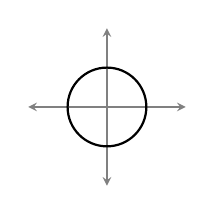
\begin{tikzpicture}[scale=0.5]
					\draw[<->, gray] (-2, 0) -- (2, 0);
					\draw[<->, gray] (0, -2) -- (0, 2);
					\draw[thick] (0, 0) circle (1);
				\end{tikzpicture}
			\end{center}
		\item\pause Two intersecting lines: $xy = 0$.
			\begin{center}
				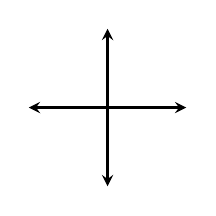
\begin{tikzpicture}[scale=0.5]
					\draw[thick, <->] (-2, 0) -- (2, 0);
					\draw[thick, <->] (0, -2) -- (0, 2);
				\end{tikzpicture}
			\end{center}
	\end{itemize}
\end{frame}

\begin{frame}
	\frametitle{Intersections of Algebraic Curves}
	\begin{itemize}
		\item One question we can ask about algebraic curves is when two of them intersect.
		
		\item\pause For example, consider the lines $x - y = 0$ and $x + 2y - 3 = 0$.
		
		\item\pause There are two ways we can find the intersection:
			\begin{center}
				\begin{tabular}{cc}
					Algebra & Picture\pause\\
					$
					\begin{cases}
						x - y = 0\\
						x + 2y - 3 = 0
					\end{cases}
					$ \pause & \raisebox{-1.4cm}{
					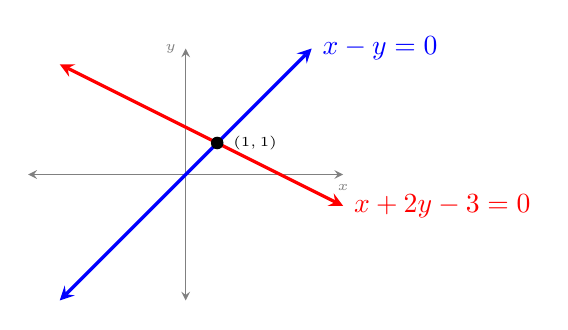
\begin{tikzpicture}[scale=0.4]
						\draw[<->, gray] (-5, 0) -- (5, 0) node[below] {\tiny$x$};
						\draw[<->, gray] (0, -4) -- (0, 4) node[left] {\tiny$y$};
						\draw[very thick, <->, blue] (-4, -4) -- (4, 4) node[right] {$x - y = 0$};
						\draw[very thick, <->, red] (-4, 3.5) -- (5, -1) node[right] {$x + 2y - 3 = 0$};
						\fill (1, 1) circle (0.2);
						\node[right] at (1.2, 1) {\tiny$(1, 1)$};
					\end{tikzpicture}}
				\end{tabular}
			\end{center}
		
		\item\pause Either way, we find that there is one intersection point: $(1, 1)$.
	\end{itemize}
\end{frame}

\begin{frame}
	\frametitle{Intersections of Algebraic Curves}
	\begin{itemize}
		\item Another example: consider the lines $2x + y - 5 = 0$ and $4x + 2y + 3 = 0$.
		
		\item\pause We could try the same methods as before:
			\begin{center}
				\begin{tabular}{cc}
					Algebra & Picture\pause\\
					$
					\begin{cases}
						2x + y - 5 = 0\\
						4x + 2y + 3 = 0
					\end{cases}
					$ \pause & \raisebox{-1.8cm}{
						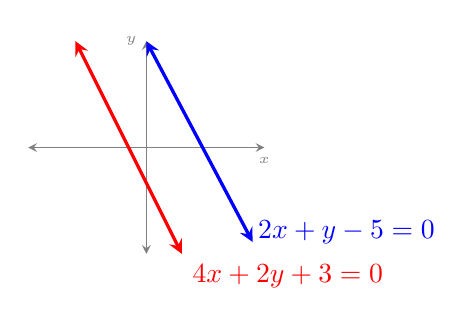
\begin{tikzpicture}[scale=0.3]
							\draw[<->, gray] (-5, 0) -- (5, 0) node[below] {\tiny$x$};
							\draw[<->, gray] (0, -4.5) -- (0, 4.5) node[left] {\tiny$y$};
							\draw[very thick, <->, blue] (0, 4.5) -- (4.5, -4) node[right, pos=0.95] {$2x + y - 5 = 0$};
							\draw[very thick, <->, red] (-3, 4.5) -- (1.5, -4.5) node[below right] {$4x + 2y + 3 = 0$};
						\end{tikzpicture}}
				\end{tabular}
			\end{center}
		
		\item\pause This time, we don't get any intersection because the lines are parallel.
	\end{itemize}
\end{frame}

\begin{frame}
	\frametitle{Intersections of Algebraic Curves}
	\begin{itemize}
		\item Every pair of lines falls into exactly one of the following two categories:
			\begin{enumerate}
				\item\pause The lines intersect at exactly one point.
				
				\item\pause The lines are parallel.
			\end{enumerate}
		
		\item\pause We need a way to treat these cases the same way.
		
		\item\pause In other words, a sense in which parallel lines intersect exactly once.
	\end{itemize}
\end{frame}

\section{Projective Geometry}
\begin{frame}
	\frametitle{Projective Geometry}
	\begin{definition}
		Projective 2-space, denoted $\mathbb{P}^2$, is defined as all triples of \emph{homogeneous coordinates} $(X : Y : Z)$
	\end{definition}
	\begin{itemize}
		\item\pause Homogeneous coordinates are triples representing a line through the origin in 3 dimensions. So $(X : Y : Z)$ and $(tX : tY : tZ)$ represent the same point.
		
		\item\pause The convention is to differentiate between affine and projective objects by using lowercase and uppercase letters, respectively.
	\end{itemize}
\end{frame}

\begin{frame}
	\frametitle{The Plane as a Subset of $\mathbb{P}^2$}
	\begin{itemize}
		\item Consider the collection of points $(X : Y : 1)$ in $\mathbb{P}^2$. This is exactly a copy of the affine plane.\pause
		\begin{center}
			\tdplotsetmaincoords{70}{130}
			\begin{tikzpicture}[tdplot_main_coords, scale=0.5]
				\draw[<->] (-5, 0, 0) -- (5, 0, 0) node[below] {$x$};
				\draw[<->] (0, -5, 0) -- (0, 5, 0) node[below] {$y$};
				\draw (0, 0, 0) -- (0, 0, 1);
				
				\draw[thick, dashed] (0, 0, 0) -- (-1, 1, 1);
				
				\begin{scope}[canvas is yx plane at z=1]
					\fill[gray, opacity=0.75] (-4.5, -4.5) rectangle (4.5, 4.5);
					\node[left] at (-4.5, 4.5) {$z=1$};
				\end{scope}
				
				\draw[->] (0, 0, 1) -- (0, 0, 4.5) node[left] {$z$};
				\draw[thick, dashed, ->] (-1, 1, 1) -- (-2.5, 2.5, 2.5) node[above right] {$(-1 : 1 : 1)$};
				\draw[mark=*, mark size=3, red] plot coordinates {(-1, 1, 1)};
			\end{tikzpicture}
		\end{center}
		\item\pause Here the homogeneous point $(-1 : 1 : 1)$ corresponds to the affine point $(-1, 1)$.
		
		\item\pause This works because lines through the origin can pass through the plane $z = 1$ exactly one time.
	\end{itemize}
\end{frame}

\begin{frame}
	\frametitle{Points With $Z = 0$ as Directions}
	\begin{itemize}
		\item Every other point in $\mathbb{P}^2$ has $Z = 0$, otherwise
			\[
			(X : Y : Z) = (X/Z : Y/Z : 1)
			\]
		
		\item\pause These points with $Z = 0$ are lines through the origin in the plane $z = 0$. So we can think of them as \emph{directions} on the affine plane living in $\mathbb{P}^2$.
			
			\begin{center}
				\tdplotsetmaincoords{70}{130}
				\begin{tikzpicture}[tdplot_main_coords, scale=0.5]
					\draw[<->] (-5, 0, 0) -- (5, 0, 0) node[below] {$x$};
					\draw[<->] (0, -5, 0) -- (0, 5, 0) node[below] {$y$};
					\draw (0, 0, 0) -- (0, 0, 1);
					
					\begin{scope}[canvas is xy plane at z=0]
						\draw (0, 2) arc (90:-90:2);
						\draw[thick, dashed, gray, ->] (0, 0) -- (2.59807621135, 4.5);
						\draw[mark=*, mark size=4, red] plot coordinates {(1, 1.73205080757)};
					\end{scope}
					
					\begin{scope}[canvas is xy plane at z=1]
						\fill[gray, opacity=0.5] (-4.59807621135, -4.5) rectangle (4.59807621135, 4.5);
						\node[left] at (4.5, -4.5) {$z=1$};
						\draw[thick, <->] (-4.59807621135, -4.5) -- (2.59807621135 - 2, 4.5);
						\draw[thick, <->] (-2.59807621135, -4.5) -- (2.59807621135, 4.5);
						\draw[thick, <->] (-0.59807621135, -4.5) -- (4.59807621135, 4.5);
					\end{scope}
					
					\draw[->] (0, 0, 1) -- (0, 0, 4.5) node[left] {$z$};
				\end{tikzpicture}
			\end{center}
		
		\item\pause These points are often called \emph{points at infinity}.
	\end{itemize}
\end{frame}

\begin{frame}
	\frametitle{Homogeneous Polynomials}
	\begin{itemize}
		\item We know how to go between coordinates -- given $(x, y)$ in the plane, the corresponding point in $\mathbb{P}^2$ is $(X : Y : 1)$.\pause\ In fact, we can make a similar construction for polynomials.
		
		\item\pause Take a polynomial in $x$ and $y$ and  ``fill in the gaps'' to create a homogeneous polynomial in $X$, $Y$, and $Z$.
		
		\item\pause For example,
			\begin{align*}
				x^2 + y - 2 &\leadsto X^2 + YZ - 2Z^2\\
				x^5y - 3xy^3 + 47y &\leadsto X^5Y - 3XY^3Z^2 + 47YZ^5
			\end{align*}
		
		\item\pause This allows us to use projective geometry to discuss algebraic curves.
	\end{itemize}
\end{frame}

\begin{frame}
	\frametitle{Intersections of Homogeneous Polynomials}
	\begin{itemize}
		\item Now that we have homogeneous polynomials, we can ask about how they intersect and how this differs from the polynomials we had before.
		
		\item\pause First, it is important to distinguish the two different ways for homogeneous polynomials to share a root.
			\begin{enumerate}
				\item\pause The root has the form $(X : Y : 1)$, in which case $(x, y)$ is a shared root of the corresponding affine polynomial.
				
				\item\pause The root has the form $(X : Y : 0)$.\pause\ We need to think a little bit more about what this means.
			\end{enumerate}
	\end{itemize}
\end{frame}

\begin{frame}
	\frametitle{Intersections of Homogeneous Polynomials (with $Z = 0$)}
	\begin{itemize}
		\item Let's go back to the example of the parallel lines from before.
		
		\item\pause Recall that the lines were defined by
			\[
			2x + y - 5 = 0 \qquad \text{and} \qquad 4x + 2y + 3 = 0
			\]
		
		\item\pause The corresponding homogeneous polynomials are
			\[
			2X + Y - 5Z = 0 \qquad \text{and} \qquad 4X + 2Y + 3Z = 0
			\]
		
		\item\pause We know that these don't have any shared points with $Z = 1$, because such a point would be an intersection of the two lines.
		
		\item\pause So let's think about $Z = 0$. Then we want to find a solution to the pair of equations
			\[
			\begin{cases}
				2X + Y = 0\\
				4X + 2Y = 0
			\end{cases}
			\]
		
		\item\pause $X = -1$, $Y = 2$ is a solution, so $(-1 : 2 : 0)$ is a shared root of our homogeneous lines.
	\end{itemize}
\end{frame}

\begin{frame}
	\frametitle{Intersecting at Infinity}
	\begin{itemize}
		\item We said before that projective points with $Z = 0$ can be thought of as \emph{points at infinity}, or as \emph{directions}. So what does it mean if two polynomials share one as a vanishing point?
		
		\item\pause It means, in some sense, that the polynomials share a direction rather than a point.
		
		\item\pause This allows us to treat the case of parallel lines the same way we treat a pair of non-parallel lines
			\begin{itemize}
				\item\pause The non-parallel lines share an affine point.
				
				\item\pause The parallel lines share a point at infinity, i.e. they share a direction.
				
				\item\pause This coincides nicely with the idea of being parallel, which really means that the lines are going in the same direction.
			\end{itemize}
	\end{itemize}
\end{frame}

\section{Intersection Multiplicity}
\begin{frame}
	\frametitle{Intersection Multiplicity}
	\begin{itemize}
		\item \onslide<+->{Another problem we could have is \emph{tangent intersections}.}
			\begin{center}
				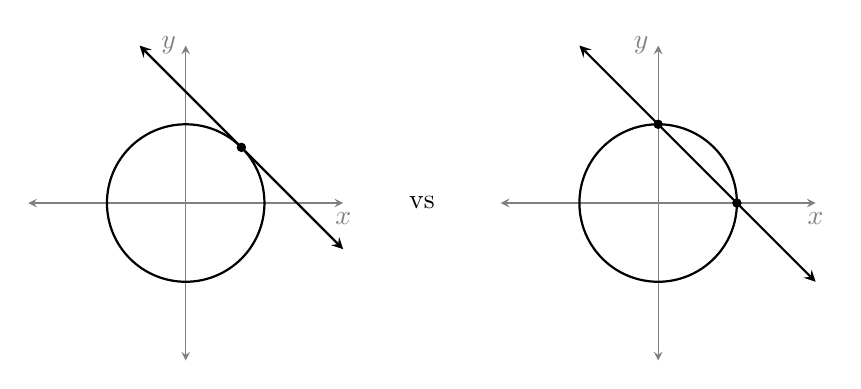
\begin{tikzpicture}[scale=0.5]
					\onslide<+->{\draw[gray, <->] (-4, 0) -- (4, 0) node[below] {$x$};
					\draw[gray, <->] (0, -4) -- (0, 4) node[left] {$y$};}
					
					\onslide<+->{\draw[thick] (0, 0) circle (2);}
					\onslide<+->{\draw[thick, <->] (-1.17157287525, 4) -- (4, -1.17157287525);
					\fill (1.41421356237, 1.41421356237) circle (0.06/0.5);}
					
					\onslide<+->{\node at (6, 0) {vs};}
					
					\begin{scope}[shift={(12, 0)}]
						\onslide<+->{\draw[gray, <->] (-4, 0) -- (4, 0) node[below] {$x$};
						\draw[gray, <->] (0, -4) -- (0, 4) node[left] {$y$};}
						
						\onslide<+->{\draw[thick] (0, 0) circle (2);}
						\onslide<+->{\draw[thick, <->] (-2, 4) -- (4, -2);
						\fill (0, 2) circle (0.06/0.5);
						\fill (2, 0) circle (0.06/0.5);}
					\end{scope}
				\end{tikzpicture}
			\end{center}
		\item \onslide<+->{The way we resolve this is \emph{intersection multiplicity}.} \onslide<+->{This is similar to the multiplicity of roots of polynomials.}
		
		\item \onslide<+->{The more two curves look like each other at an intersection point, the higher the intersection multiplicity of that point is.}
	\end{itemize}
\end{frame}

\section{Bezout's Theorem}
\begin{frame}
	\frametitle{Bezout's Theorem}
	\begin{itemize}
		\item We are finally ready to state Bezout's Theorem!\pause
			\begin{theorem}[Bezout's Theorem]
				If $p(x, y)$ and $q(x, y)$ are two polynomials of respective degrees $n$ and $m$, then the algebraic curves defined by $p = 0$ and $q = 0$ intersect at exactly $nm$ points, accounting for complex roots, intersections at infinity, and intersection multiplicity.
			\end{theorem}
		
		\item\pause It is clear now that we need all the conditions in the theorem in order for it to hold:
			\begin{itemize}
				\item\pause If we don't allow for complex roots, some polynomials may not have any roots at all, so the corresponding algebraic curves will be empty.
				
				\item\pause If we don't consider intersections at infinity, some algebraic curves will not intersect.
				
				\item\pause If we don't consider intersection multiplicity, the number of intersections will be counted as too low.
			\end{itemize}
	\end{itemize}
\end{frame}
\section{The Group Law on Cubics}
\begin{frame}
	\frametitle{The Group Law on Cubics}
	\begin{itemize}
		\item \onslide<+->{A \emph{cubic} is a polynomial whose largest term has degree three.}
			\begin{center}
				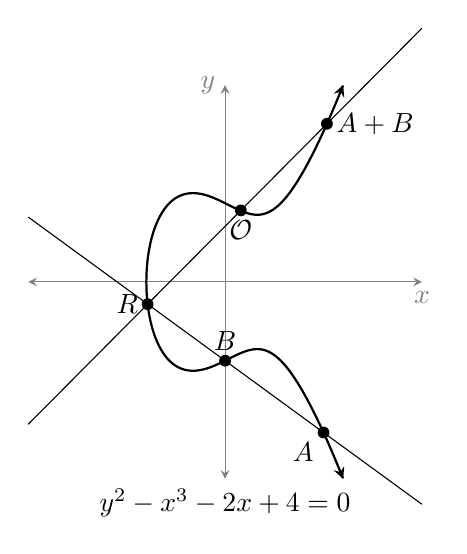
\begin{tikzpicture}[scale=0.5]
					\onslide<+->{\draw[gray, <->] (-5, 0) -- (5, 0) node[below] {$x$};
					\draw[gray, <->] (0, -5) -- (0, 5) node[left] {$y$};}
					
					\onslide<+->{\draw[smooth, domain=-2:3, ->, thick, samples=1000] plot (\x, {sqrt(\x * \x * \x - 2 * \x + 4)});
					\draw[smooth, domain=-2:3, ->, thick, samples=1000] plot (\x, {-sqrt(\x * \x * \x - 2 * \x + 4)});
					
					\node[below] at (0, -5) {$y^2 - x^3 - 2x + 4 = 0$};}
					
					\onslide<+->{\fill (0.4, 1.817) circle (0.15);
					\node[below] at (0.4, 1.817) {$\mathcal{O}$};}
					
					\onslide<+->{\fill (2.5, -3.824) circle (0.15);
					\node[below left] at (2.5, -3.824) {$A$};}
					
					\onslide<+->{\fill (0, -2) circle (0.15);
					\node[above] at (0, -2) {$B$};}
					
					\onslide<+->{\draw (-5, 1.648) -- (5, -5.648);}
					
					\onslide<+->{\fill (-1.968, -0.565) circle (0.15);
					\node[left] at (-1.968, -0.565) {$R$};}
					
					\onslide<+->{\draw (-5, -3.61491) -- (5, 6.44419);}
					
					\onslide<+->{\fill (2.587, 4.017) circle (0.15);
					\node[right] at (2.587, 4.017) {$A + B$};}
				\end{tikzpicture}
			\end{center}
		\item \onslide<+->{It is convenient to take $\mathcal{O} = (0 : 1 : 0)$ because this is a vertical line.}
	\end{itemize}
\end{frame}

\begin{frame}
	\frametitle{The End}
	\centering\huge Thank you!
\end{frame}

\end{document}